\chapter{Opis środowiska}
W celu uniknięcia konieczności zajmowania się niskopoziomowymi problemami, takimi jak:
\begin{itemize}
    \item zrównoleglanie obliczeń wektorowych,
    \item wykonywanie obliczeń na~karcie graficznej,
    \item liczenie gradientów operacji wykonywanych przez sieć neuronową (takich jak~sploty, normalizacje, aktywacje),
    \item wczytywanie danych,
    \item itp.
\end{itemize}
postanowiono skorzystać z~jednej~z~dostępnych bibliotek, która zajmuje się~owymi zagadnieniami. Pozwala to~na~skupienie
się~na~architekturze sieci oraz na odpowiednim doborze operacji mających na~celu zapewnienie jak~najlepszej
klasyfikacji.

\section{Wybrana biblioteka}
Do~realizacji badań wykonywanych w~ramach niniejszej pracy magisterskiej wykorzystano bibliotekę
\textbf{Tensorflow} firmy Google.

W~rozdziale opisano podstawowe zagadnienia dotyczące wybranego narzędzia. Wiedza ta~pozwoli na~zrozumienie
informacji o~architekturze sieci przedstawianych w~dalszych częściach pracy.

\section{Graf operacji}
Tworzenie sztucznej sieci neuronowowej przy~użyciu wymienionej powyżej biblioteki, można podzielić na~dwa etapy:
\begin{enumerate}
    \item zdefiniowanie grafu operacji,
    \item wykonanie wybranych operacji z~grafu.
\end{enumerate}

Graf operacji definiuje w~jaki sposób dane wejściowe mają być przetwarzane po to, by osiągnąć rezultat na wyjściu.
Każda operacja może przyjmować pewne dane wejściowe. Dane wejściowe mogą być zarówno danymi wczytanymi z~dysku
czy~z~klawiatury. Najczęściej jednak są one~wynikami innych operacji. W~ten sposób operacje tworzą wzajemne zależności,
gdzie wyjście jednej z~nich jest jednocześnie wejściem innej. Operacje mogą być ze sobą grupowane poprzez tworzenie
tzw.~zakresów (\textit{ang.~scope}). Przykładowy graf przedstawiono na rysunku \ref{img:tf-smpl-grf}.

\begin{figure}[H]
	\centering
	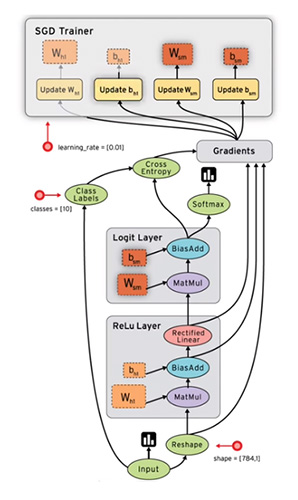
\includegraphics[width=0.5\linewidth]{img/tf-sample-graph.jpg}
	\caption{Przykładowy graf operacji}
	\label{img:tf-smpl-grf}
\end{figure}

\subsection{Konstrukcja grafu}
W pierwszym etapie tworzenia sieci neuronowej należy zdefiniować graf operacji. W~następnym kroku można wykonać
wybrane operacje, a~silnik Tensorflow sam wykona wszystkie akcje wymagane do~poprawnego obliczenia ich rezultatu.

Podczas konstrukcji grafu zamiast konkretnych danych wykorzystywane są dane symboliczne (np.~,,zmienna~x'',
,,dana~C''). Dopiero później, w etapie wykonania operacji, za~niektóre z~owych danych podstawiane
są~odpowiednie wartości (podczas wykonywania operacji do~silnika Tensorflow podawany jest tzw.~kontekst będący
słownikiem odwzorowującym wybrane dane symboliczne na realne wartości).

\pythonexternal{code/graph_creation.py}

\subsection{Wykonanie operacji}
Dwoma naistotniejszymi operacjami wykonywanymi podczas konstrukcji sieci neuronowej będą:
\begin{itemize}
    \item operacja uczenia,
    \item operacja klasyfikacji.
\end{itemize}

Mając już skonstruowany graf operacji, można wykonać dowolną operację zdefiniowaną w~grafie (np.~operację klasyfikacji).

\pythonexternal{code/op_execution.py}
